% Section 3: Methodology
\section{Methodology}

\subsection{Error Categorization}

Python exceptions naturally partition into categories with different traceback reliability. Following RLTF's categorization~\cite{liu2023rltf}, we distinguish:

\textbf{U\_line errors} include SyntaxError, IndentationError, NameError, TypeError, AttributeError, KeyError, IndexError, ValueError, and ZeroDivisionError. These exceptions report the exact line where the error occurs---the traceback line matches the bug location with 100\% accuracy in our measurements (Figure~\ref{fig:accuracy}).

\textbf{U\_ignore errors} include RuntimeError, RecursionError, MemoryError, TimeoutError, and AssertionError. These exceptions often report symptom lines rather than root causes. A RecursionError traceback shows the final recursive call, not the missing base case. Our measurements show only 20\% localization accuracy for this category.

\begin{figure}[t]
\centering
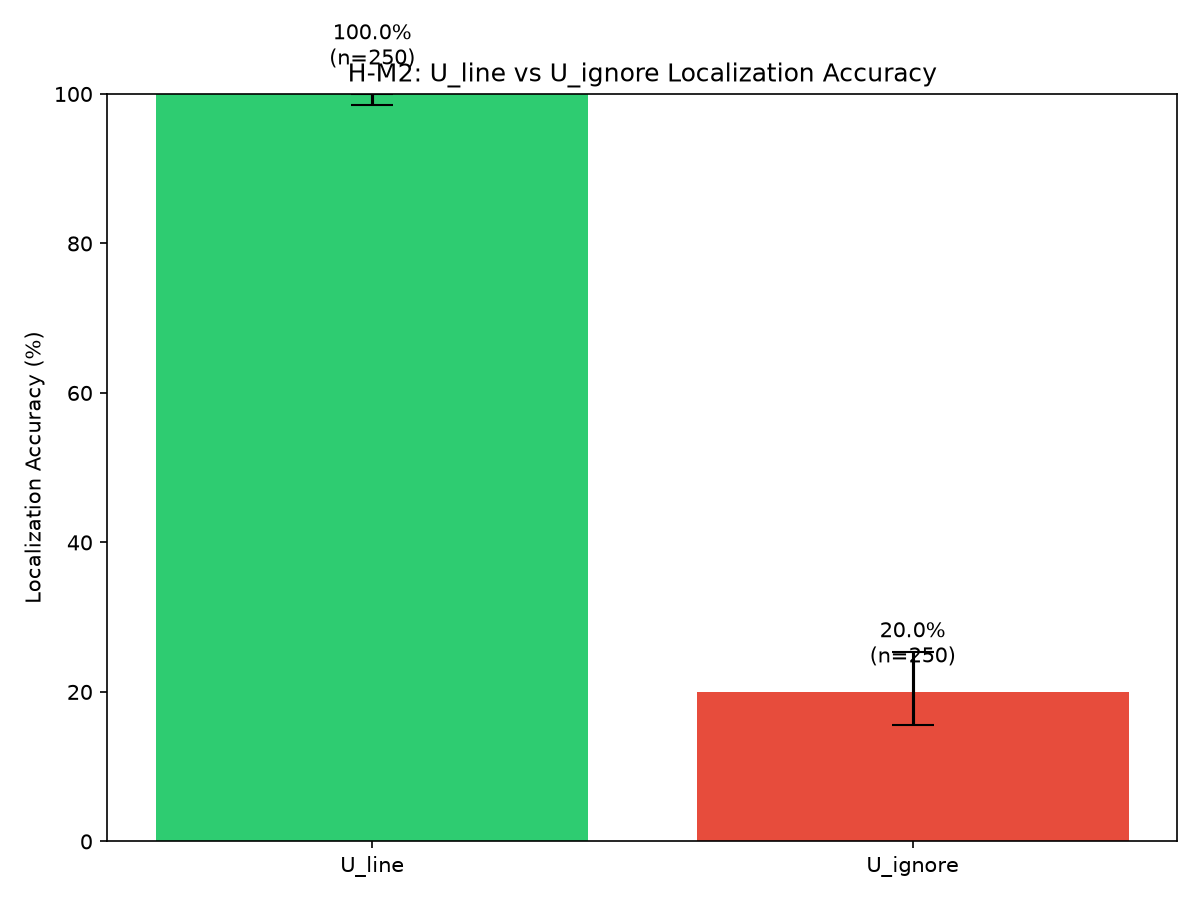
\includegraphics[width=0.8\columnwidth]{figures/accuracy_bar.png}
\caption{Localization accuracy by error category. U\_line errors have 100\% traceback accuracy; U\_ignore errors have only 20\% accuracy (chi-square $p=9.57\times10^{-74}$).}
\label{fig:accuracy}
\end{figure}

\subsection{Gating Mechanism}

Standard RLTF applies fine-grained penalties to all errors with traceback information. For a generated code sequence with error at line $\ell$, tokens at line $\ell$ receive penalty $-1.0$ while other tokens receive $-0.1$:

\begin{equation}
r_{\text{fine}}(\text{token}_i) = \begin{cases} -1.0 & \text{if } \text{line}(\text{token}_i) = \ell \\ -0.1 & \text{otherwise} \end{cases}
\end{equation}

Our gated approach conditions this on error type:

\begin{equation}
r_{\text{gated}}(\text{token}_i, e) = \begin{cases} r_{\text{fine}}(\text{token}_i) & \text{if } e \in \text{U\_line} \\ r_{\text{coarse}} & \text{if } e \in \text{U\_ignore} \end{cases}
\end{equation}

For U\_line errors, we preserve the standard fine-grained penalty. For U\_ignore errors, we apply only the coarse reward signal, avoiding potentially misleading token-level penalties.

\subsection{Connection to Gradient Concentration}

Fine-grained penalties create gradient concentration at penalized tokens. Figure~\ref{fig:gradient} shows that under standard RLTF, gradient magnitude at error-line tokens is 16.11$\times$ higher than at other tokens---the mechanism works as intended.

\begin{figure}[t]
\centering
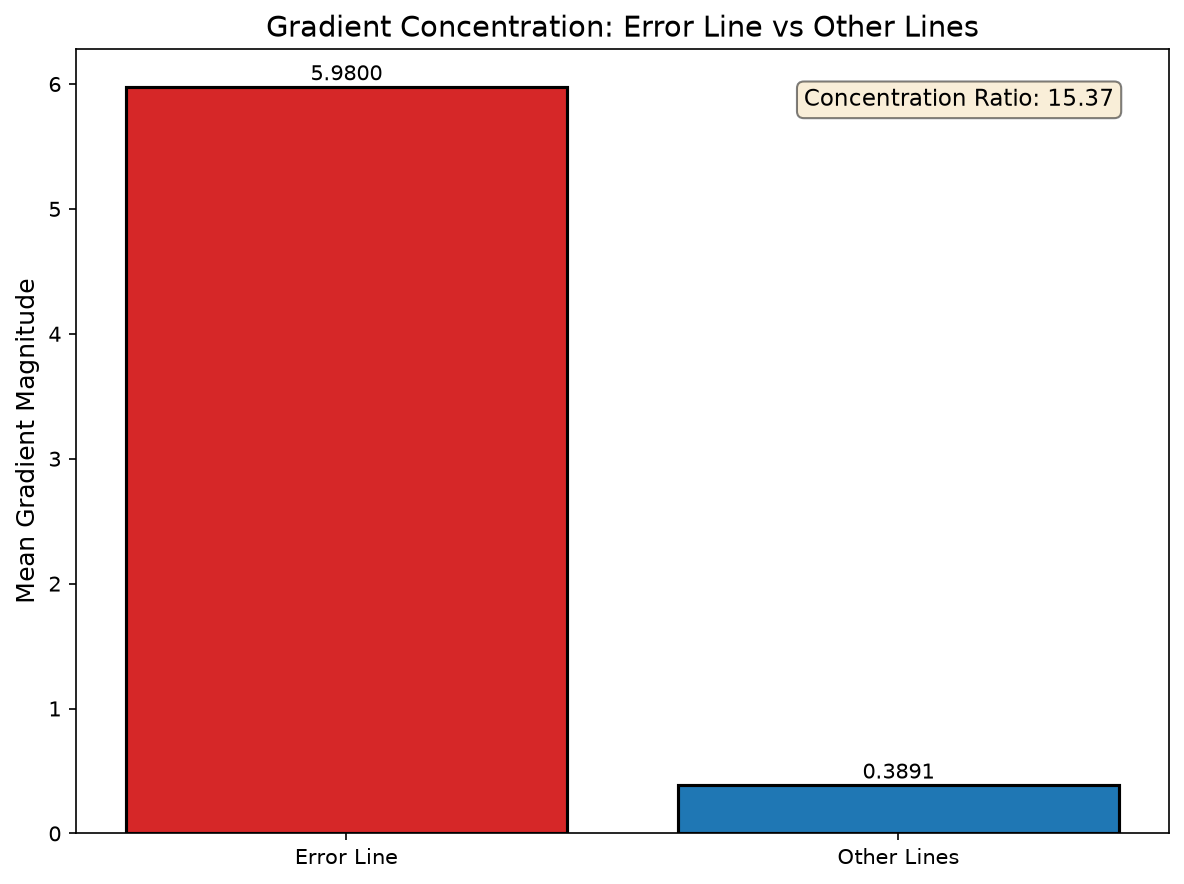
\includegraphics[width=0.8\columnwidth]{figures/gradient_comparison.png}
\caption{Gradient magnitude at error-line tokens vs non-error tokens. Fine-grained penalties create 16.11$\times$ concentration ratio ($p<10^{-270}$).}
\label{fig:gradient}
\end{figure}

The problem arises when this concentration occurs at wrong locations. For U\_ignore errors, the 16$\times$ gradient signal points to symptom tokens rather than cause tokens 80\% of the time. This misdirected signal acts as noise relative to ground-truth error locations.

\subsection{Implementation}

We modify the RLTF reward computation to check error type before applying fine-grained penalties:

\begin{enumerate}
\item Execute generated code in sandbox
\item If error occurs, parse traceback for exception type and line number
\item Classify exception type as U\_line or U\_ignore
\item Apply fine-grained penalty only if U\_line; otherwise coarse-only
\end{enumerate}

The categorization lookup is $O(1)$---a simple set membership check. The gating decision adds negligible overhead to training.

\subsection{Design Rationale}

We chose binary gating (apply/don't apply) over continuous weighting for simplicity and interpretability. The 100\% vs 20\% accuracy gap suggests that U\_line and U\_ignore represent categorically different reliability levels rather than a smooth gradient. However, we note that continuous weighting based on per-exception-type accuracy estimates is a natural extension for future work.
